\section{Screening of the phonon-assisted rate}\label{sec:13.4}

The loss function of \cref{sec:13.3} uses the bare density vertex. At a momentum transfer of \SI{1}{keV} and an energy of \SI{1.2}{eV}, inside the phonon-assisted window, however, the dielectric function of silicon is about 6 in the random-phase approximation (\cref{we:13-external}). The potential that the dark matter exerts on a valence electron is therefore six times weaker than the bare one, and the bare loss function is too large by a factor of 30 to 50. Screening enters the amplitude of \cref{sec:13.2} at three places, among which \cref{sec:8.4} sorted the Coulomb lines: the dark-matter vertex at $(\vect{q},\omega)$, the electron--phonon vertex at $(\vect{Q},\omega_{\vect{Q}\nu})$, and the final pair at $(\vect{q}+\vect{Q}, \omega \mp \omega_{\vect{Q}\nu})$. With all three in the amplitude, the loss function keeps one macroscopic factor $1/\varepsilon_{\mathrm{mac}}(\vect{q},\omega)^2$ and nothing else outside it; \cref{app:D.36} gives the steps at the random-phase level.

\subsection{The screened density and phonon vertices}

The electron--phonon vertex is already screened. Density-functional perturbation theory returns $g_{mn\nu}(\vect{k},\vect{Q})$ as the matrix element of the self-consistent potential change $\partial V_{\mathrm{KS}}$, which is the bare potential of the displaced ions dressed by every Coulomb chain at $\vect{Q}+\vect{G}$, the operator $(1 - f_{\mathrm{Hxc}}R^0)^{-1}$ of \cref{eq:6.2-screen}. These are the vertex lines of \cref{sec:8.4-lines}. The calculation evaluates them at zero frequency, although they carry the phonon frequency; below the gap the error is of relative order $(\omega_{\vect{Q}\nu}/\Eg)^2$, about $3\times10^{-3}$ in silicon (\cref{sec:8.4-lines}). Dividing the computed $g$ once more by $\varepsilon(\vect{Q})$ would count these lines twice, and a bare ionic potential in its place would overstate the long-range part of the coupling by about $\varepsilon_\infty$.

The density vertex of \cref{eq:13.2-M} is bare. The dark matter applies a potential at $(\vect{q},\omega)$, and the electrons that it polarizes add their Hartree and exchange--correlation potentials at every $\vect{q} + \vect{G}$. An electron feels the total, the external potential times the column $(\tilde\varepsilon^{-1})_{\vect{G}0}(\vect{q},\omega)$ of the inverse dielectric matrix of a test electron (\cref{sec:8.7}). These are the external lines, and in the amplitude they replace the density vertex by
\begin{equation}
  \rho^{\mathrm{scr}}_{mn}(\vect{k},\vect{q}) = \sum_{\vect{G}}\bigl(\tilde\varepsilon^{-1}\bigr)_{\vect{G}0}(\vect{q},\omega)\,\rho_{mn}(\vect{k},\vect{q}+\vect{G}) ,
  \label{eq:13.4-rhoscr}
\end{equation}
the vertex of the total potential, as in the screened pair weight \cref{eq:8.7-screened}. The sum over $\vect{G}$ carries the local fields. Without local fields, where the dielectric matrix is diagonal, and without an exchange--correlation kernel, $\rho^{\mathrm{scr}}$ is $\rho/\varepsilon_{\vect{0}\vect{0}}(\vect{q},\omega)$, the head screening of \cref{sec:10.2}.

Exactly one factor of $1/\varepsilon$ survives once the local fields are kept. To see this, remove from the Coulomb kernel its macroscopic term, $v_{\mathrm{C}}(q)$ at $\vect{G} = \vect{G}' = 0$, and let $\bar R$ be the response without it (\cref{sec:4.4}). The full response is then $\bar R$ plus chains of $\bar R$ joined by the macroscopic line, and each element $(\tilde\varepsilon^{-1})_{\vect{G}0}$ factors into $(\varepsilon^{-1})_{\vect{0}\vect{0}} = 1/\varepsilon_{\mathrm{mac}}$ times a local-field column (\cref{app:D.36}). In the random-phase approximation,
\begin{equation}
  \begin{aligned}
  \rho^{\mathrm{scr}}_{mn}(\vect{k},\vect{q}) &= \frac{\rho^{\mathrm{LF}}_{mn}(\vect{k},\vect{q})}{\varepsilon_{\mathrm{mac}}(\vect{q},\omega)} , \\
  \rho^{\mathrm{LF}}_{mn}(\vect{k},\vect{q}) &= \rho_{mn}(\vect{k},\vect{q}) + \sum_{\vect{G}\ne0}v_{\mathrm{C}}(|\vect{q}+\vect{G}|)\,\bar R_{\vect{G}0}(\vect{q},\omega)\,\rho_{mn}(\vect{k},\vect{q}+\vect{G}) ,
  \end{aligned}
  \label{eq:13.4-rhoLF}
\end{equation}
exactly, with $\varepsilon_{\mathrm{mac}}$ the macroscopic dielectric function \cref{eq:4.4-epsmac}. An exchange--correlation kernel adds its own elements, its head included, to the local-field vertex $\rho^{\mathrm{LF}}$ and leaves the factorization intact. Physically, $\rho^{\mathrm{LF}}$ is the bare vertex corrected by the microscopic potentials that the macroscopic field induces inside each cell, and $1/\varepsilon_{\mathrm{mac}}$ is the reduction of the macroscopic field itself. Without local fields $\rho^{\mathrm{LF}} = \rho$ and $\varepsilon_{\mathrm{mac}} = \varepsilon_{\vect{0}\vect{0}}$.

Inside the window this factor is real. No zero-phonon pair exists at $(\vect{q},\omega)$, so the independent-particle response at that momentum and energy has no absorptive part, and $\varepsilon_{\mathrm{mac}}(\vect{q},\omega)$ is real up to the phonon-assisted terms of order $g^2$ that this section computes. We write its zero-phonon value $\varepsilon_1^0(\vect{q},\omega)$, the real part of $\varepsilon_{\mathrm{mac}}$ at $n_g = 0$; its imaginary part $\varepsilon_2^0$ vanishes in the window. The response $R(\vect{q},\omega)$ is then Hermitian, so the retarded column $\delta_{\vect{G}0} + (f_{\mathrm{Hxc}}R)_{\vect{G}0}$ and the advanced one $\delta_{\vect{G}0} + (f_{\mathrm{Hxc}}R^\dagger)_{\vect{G}0}$ coincide, and the question of \cref{sec:8.7}, which of the retarded and advanced weights labels a final pair, does not arise for the external lines. It arises at the pair.

\subsection{The pair channel}

Once the phonon has taken the momentum $\vect{Q}$, the dark matter and the phonon together have disturbed the electrons at a third wavevector, $\vect{q} + \vect{Q}$, and at a third frequency,
\begin{equation*}
  \omega_f = \omega \mp \omega_{\vect{Q}\nu} ,
\end{equation*}
the upper sign for emission. These are the crystal momentum and energy of the final pair itself, $\varepsilon_{c,\vect{k}+\vect{q}+\vect{Q}} - \varepsilon_{v\vect{k}} = \omega_f$ on shell. The disturbance is a density of second order, bilinear in the two vertices, and its Hartree and exchange--correlation potential acts back on the electrons at $(\vect{q}+\vect{Q}+\vect{G},\omega_f)$. That potential can create the final pair directly. Summed over the chains that the medium inserts, it is the pair channel of \cref{sec:8.4-lines}: the Coulomb lines on the segment of the cycle between the two dark-matter vertices. The four-path amplitude of \cref{sec:13.2} leaves it out, because it treats the electrons as independent once the two vertices are given.

To find it we follow the density matrix $\varrho$ of the Kohn--Sham electrons to second order in time-dependent mean-field theory (\cref{app:D.36}). The dark matter acts through the screened vertex, $\mathsf{x} = \rho^{\mathrm{scr}}$ at frequency $\omega$, and the phonon through $\mathsf{y} = g$ at frequency $\mp\omega_{\vect{Q}\nu}$, with the factor $N^{-1/2}(n_{\vect{Q}\nu} + \frac12 \pm \frac12)^{1/2}$ of \cref{eq:13.2-M} taken out. Each field alone produces a first-order density matrix, $\varrho^{\mathsf{x}}_{ab} = \mathsf{x}_{ab}(f_b - f_a)/(\omega - \varepsilon_a + \varepsilon_b + \ii0^+)$ and its analog $\varrho^{\mathsf{y}}$, with $f_a$ the occupation of the one-electron state $a$. At second order, each field acts on the first-order response to the other, which gives the source
\begin{equation*}
  \mathfrak{s}^{(2)}_{ab} = \sum_m\bigl[\mathsf{x}_{am}\varrho^{\mathsf{y}}_{mb} - \varrho^{\mathsf{y}}_{am}\mathsf{x}_{mb} + \mathsf{y}_{am}\varrho^{\mathsf{x}}_{mb} - \varrho^{\mathsf{x}}_{am}\mathsf{y}_{mb}\bigr] ,
\end{equation*}
a matrix over every pair of states, filled or empty. Its element between the final conduction state and the final valence state is, on shell, the four-path amplitude itself, $\mathfrak{s}^{(2)}_{cv} = M^\pm[\rho^{\mathrm{scr}}]$, \cref{eq:13.2-M} with the screened vertex and the unrestricted band sum: the hole paths enter through the occupation differences, and the band-sum theorem of \cref{app:D.35} follows from the density matrix without Fock space.

The source drives a second-order density of the Kohn--Sham electrons at $\vect{q}+\vect{Q}+\vect{G}$,
\begin{equation}
  \delta\nd^{(2)}_{\vect{G}}(\vect{q}+\vect{Q}) = \frac{2}{\Vol}\sum_{\vect{k}}\sum_{ab}\frac{\rho_{ab}(\vect{k},\vect{q}+\vect{Q}+\vect{G})^*\,\mathfrak{s}^{(2)}_{ab}(\vect{k})}{\omega_f + \varepsilon_{b\vect{k}} - \varepsilon_{a,\vect{k}+\vect{q}+\vect{Q}} + \ii0^+} ,
  \label{eq:13.4-dn2}
\end{equation}
the sum running over all pairs of states, including the rearrangements among filled and among empty bands. Its potential is screened by the same chains as any potential at that wavevector and frequency: the electrons respond to it with the bubble $R^0(\vect{q}+\vect{Q},\omega_f)$, their response adds potential, and the series sums to $\tilde\varepsilon^{-1}f_{\mathrm{Hxc}}\,\delta\nd^{(2)}$. In the random-phase approximation $\tilde\varepsilon^{-1}f_{\mathrm{Hxc}} = \varepsilon^{-1}v_{\mathrm{C}}$ is the retarded screened interaction $W^{\mathrm{scr,R}}$ of \cref{eq:4.8-W}. The equation of motion of the pair element $\varrho^{(2)}_{cv}$ is that of a first-order coherence driven at $\omega_f$ by $\mathfrak{s}^{(2)}$ plus this potential, and its numerator is the amplitude for creating the pair. Finally, every term is linear in $\mathsf{x}$, so the factor $1/\varepsilon_{\mathrm{mac}}(\vect{q},\omega)$ of \cref{eq:13.4-rhoLF} comes out in front.
\begin{keyresult}[Screened phonon-assisted amplitude]
In the random-phase approximation and at order $g$ in the amplitude, the screened matrix element of the density into the final state \cref{eq:13.2-final} is $N^{-1/2}(n_{\vect{Q}\nu} + \frac12 \pm \frac12)^{1/2}\,\tilde M^\pm_{cv\nu}(\vect{k},\vect{q},\vect{Q})/\varepsilon_{\mathrm{mac}}(\vect{q},\omega)$. The amplitude without the macroscopic factor is
\begin{equation}
  \begin{split}
  \tilde M^\pm_{cv\nu}(\vect{k},\vect{q},\vect{Q}) &= M^\pm_{cv\nu}\bigl[\rho^{\mathrm{LF}}\bigr] + \sum_{\vect{G}\vect{G}'}\rho_{cv}(\vect{k},\vect{q}+\vect{Q}+\vect{G})\\
  &\quad\times W^{\mathrm{scr,R}}_{\vect{G}\vect{G}'}(\vect{q}+\vect{Q},\omega_f)\,\delta\nd^{(2)}_{\vect{G}'}(\vect{q}+\vect{Q}) ,
  \end{split}
  \label{eq:13.4-Mscr}
\end{equation}
where $M^\pm[\rho^{\mathrm{LF}}]$ is \cref{eq:13.2-M} with the local-field vertex \cref{eq:13.4-rhoLF}, $\delta\nd^{(2)}$ is \cref{eq:13.4-dn2} built with $\mathsf{x} = \rho^{\mathrm{LF}}$, and the retarded $W^{\mathrm{scr,R}}$ carries the index of the final pair first. With an exchange--correlation kernel, $W^{\mathrm{scr,R}}$ becomes $\tilde\varepsilon^{-1}f_{\mathrm{Hxc}}$, and an adiabatic local kernel adds the source of \cref{eq:13.4-kxc}.
\end{keyresult}
\noindent The pair-channel term is added to the four-path term, not multiplied: it does not rescale the four-path term by $1/\varepsilon(\vect{q}+\vect{Q},\omega_f)$, and no $1/|\varepsilon|^4$ appears anywhere. The rate needs \cref{eq:13.4-Mscr} only on shell, where $\mathfrak{s}^{(2)}_{cv}$ equals the four-path amplitude.

\Cref{fig:13-screening} shows the three kinds of screening as diagrams. With the external chains at $(\vect{q},\omega)$, the static chains inside $g$ and the pair chain at $(\vect{q}+\vect{Q},\omega_f)$, every random-phase diagram with one phonon in the final state is counted once (\cref{sec:8.4-lines}). The classification is by the position of a line on the diagram, so it holds where the momentum labels coincide.

\begin{figure}[tbp]
  \centering
  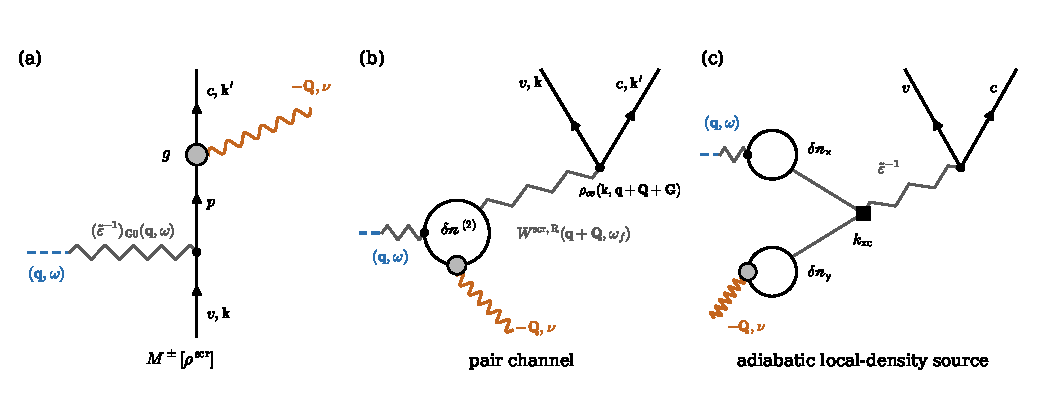
\includegraphics[width=\linewidth]{figures/ch13/fig13_4.pdf}
  \caption{Screening of the phonon-assisted amplitude, schematic. Time runs upward; solid lines are electrons and holes, dashed blue lines the dark-matter potential, wavy lines the phonon, and zigzag lines Coulomb chains summed to all orders. (a) The four-path term $M^\pm[\rho^{\mathrm{scr}}]$: the dark-matter potential reaches the electron through the external chains at $(\vect{q}+\vect{G},\omega)$, the column $(\tilde\varepsilon^{-1})_{\vect{G}0}(\vect{q},\omega)$, and the phonon through the vertex $g$ of density-functional perturbation theory (gray disk), whose chains at $(\vect{Q}+\vect{G},\approx0)$ are inside it. One of the four paths is drawn. (b) The pair channel: the two vertices act on a loop of Kohn--Sham electrons and produce the second-order density $\delta\nd^{(2)}$ at $(\vect{q}+\vect{Q}+\vect{G}',\omega_f)$, whose potential, screened by $W^{\mathrm{scr,R}}(\vect{q}+\vect{Q},\omega_f)$, creates the final pair through $\rho_{cv}(\vect{k},\vect{q}+\vect{Q}+\vect{G})$. (c) The extra source of an adiabatic local-density kernel: the first-order densities induced by the dark matter and by the phonon meet at one point through $k_{\mathrm{xc}}$, the third derivative of the exchange--correlation energy, and the potential they produce is screened at the pair. In the random-phase approximation panel (c) is absent.}
  \label{fig:13-screening}
\end{figure}

The pair line is complex. The final pair is on shell, so pairs exist at $(\vect{q}+\vect{Q},\omega_f)$, and the response there has an absorptive part. With an absorptive interaction the share of the total rate that each final pair receives depends on whether the retarded or the advanced interaction is used, while the total does not. The pair that the cascade receives is the out-state of the evolution, and it takes the retarded $W^{\mathrm{scr,R}}$, as the external weight did in \cref{sec:8.7}.

The momentum of the pair channel is pinned. At the threshold the hole sits near the valence maximum at $\mathrm{\Gamma}$ and the electron near the bottom of a valley at $\vect{k}_{\mathrm{c}}$. The pair momentum $\vect{q}+\vect{Q}$ therefore equals $\vect{k}_{\mathrm{c}}$ up to a reciprocal-lattice vector, whatever $\vect{q}$ is, exactly at the onset and within a few tenths of an inverse \si{\angstrom} at the top of the window. In silicon $|\vect{k}_{\mathrm{c}}| = 0.85\,(2\pi/a) = \SI{1.94}{keV}$, and $\omega_f$ lies within a few tenths of an eV of the gap. One screened interaction, at the six valley momenta and a narrow band of energies, serves the whole window; it is the same one that screens phonon-assisted optical absorption, where $\vect{q} = 0$ and the pair momentum is $\vect{Q}$ (\cref{sec:13.5}). Only $\delta\nd^{(2)}$ depends on $\vect{q}$.

Two limits can be solved, and they show what the pair channel does. In the first, the applied-potential limit, the source acts on every pair at $\vect{q}+\vect{Q}$ as an applied potential would, $\mathfrak{s}^{(2)}_{ab}$ proportional to $\rho_{ab}(\vect{k},\vect{q}+\vect{Q})(f_b - f_a)$. Then $\delta\nd^{(2)}$ is the bubble times that potential, and the two terms of \cref{eq:13.4-Mscr} combine into the source screened as an external potential at the pair's own momentum and energy, $\tilde M^\pm = M^\pm[\rho^{\mathrm{LF}}]/\varepsilon(\vect{q}+\vect{Q},\omega_f)$ without local fields (\cref{app:D.36}). In this limit the pair channel reduces the rate by $1/\varepsilon_1(\vect{k}_{\mathrm{c}},\omega_f)^2$, the screening of the final pair's own momentum.

In the second limit the phonon is a rigid translation of the crystal, $\vect{Q} = 0$, and the vertex is the commutator of the electron momentum with the Kohn--Sham Hamiltonian (\cref{eq:6.2-asr}). In the frame that moves with the nuclei the dark-matter potential only acquires a phase factor, and the displaced density is screened at the energy of the final pair, $1/\varepsilon(\vect{q},\omega_f)$. The four-path term alone gives $1/\varepsilon(\vect{q},\omega)$, screened at the energy deposited, and the pair channel supplies exactly the difference, $1/\varepsilon(\vect{q},\omega_f) - 1/\varepsilon(\vect{q},\omega)$ (\cref{app:D.36}). In the strict limit an acoustic $\omega_{\vect{Q}\nu}$ vanishes, $\omega_f = \omega$, and the pair term vanishes with it. Evaluated with the transverse acoustic energy of the window instead, the two energies change $\varepsilon_1$ of silicon by $1\times10^{-3}$ and the rate by $2\times10^{-3}$ (\cref{we:13-external}). The limit therefore tests the sign and the normalization of \cref{eq:13.4-Mscr}, not its size. It requires a zero-phonon pair at $(\vect{q},\omega_f)$ and therefore lies outside the window. Inside it, the phonons that carry the missing momentum have wavevectors near the zone boundary, where the displacement is not a translation of anything, and the pair channel is neither of these limits.

\subsection{The screened phonon-assisted loss function}

The rate follows from the screened amplitude as it followed from the bare one in \cref{sec:13.3}: the golden rule into the bare pairs, summed over $\vect{k}$, $\vect{Q}$, bands, branches and spin. That this sum is the whole absorptive part of the one-phonon response, with nothing counted twice, is the optical theorem of the mean-field evolution: cut at the pair, the diagrams with both dark-matter vertices on one loop give $|M^\pm[\rho^{\mathrm{LF}}]|^2$, and those with a pair segment the cross terms and the square of the pair channel, which together make $|\tilde M^\pm|^2$ pair by pair (\cref{app:D.36}). The amplitude therefore enters \cref{eq:13.3-LPA} with $M^\pm \to \tilde M^\pm/\varepsilon_{\mathrm{mac}}(\vect{q},\omega)$.

Write $\varepsilon_{\mathrm{mac}} = \varepsilon_1^0 + \delta\varepsilon_1 + \ii\varepsilon_2$, where $\delta\varepsilon_1$ and $\varepsilon_2$ are the phonon-assisted parts, both of order $g^2$ because $\varepsilon_2^0 = 0$. Then $|\varepsilon_{\mathrm{mac}}|^{-2} = (\varepsilon_1^0)^{-2}[1 + O(g^2)]$, and since $|\tilde M^\pm|^2$ is already of order $g^2$, every correction is of order $g^4$, the next order of the expansion in \cref{sec:8.5}.
\begin{keyresult}[Screened phonon-assisted loss function]
Inside the off-shell window, where $\varepsilon_2^0(\vect{q},\omega) = 0$,
\begin{equation}
  \begin{aligned}
  L^{\mathrm{PA}}(\vect{q},\omega) &= \frac{\varepsilon_2^{\mathrm{PA}}(\vect{q},\omega)}{\varepsilon_1^0(\vect{q},\omega)^2} + O(g^4) , \\
  \varepsilon_2^{\mathrm{PA}}(\vect{q},\omega) &= \frac{8\pi^2\alpha}{\Omega\,q^2}\,\Bigl\langle\!\Bigl\langle\sum_{\nu cv\pm}w_\pm\,\bigl|\tilde M^\pm_{cv\nu}\bigr|^2\,\delta\bigl(\varepsilon_{c,\vect{k}+\vect{q}+\vect{Q}} - \varepsilon_{v\vect{k}} \pm \omega_{\vect{Q}\nu} - \omega\bigr)\Bigr\rangle\!\Bigr\rangle ,
  \end{aligned}
  \label{eq:13.4-Lscr}
\end{equation}
with $\tilde M^\pm$ of \cref{eq:13.4-Mscr}, the weights $w_\pm$ of \cref{eq:13.3-LPA}, and $\varepsilon_1^0$ the macroscopic zero-phonon dielectric function with local fields. The rate is \cref{eq:10.2-rate} with $\bar L$ replaced by the direction average $\bar L^{\mathrm{PA}}$.
\end{keyresult}
\noindent From here on $L^{\mathrm{PA}}$ denotes this screened loss function; the function of \cref{eq:13.3-LPA} is its independent-particle value. The definition of $\varepsilon_2^{\mathrm{PA}}$ in \cref{eq:13.4-Lscr} identifies it as the imaginary part, at order $g^2$, of the macroscopic dielectric function, since $L = \Imag(-1/\varepsilon_{\mathrm{mac}}) = \varepsilon_2/|\varepsilon_{\mathrm{mac}}|^2$ must agree with the golden-rule sum term by term. \Cref{eq:13.4-Lscr} is therefore the familiar $L = \varepsilon_2/|\varepsilon|^2$ of \cref{sec:4.4}, evaluated where the zero-phonon $\varepsilon_2$ vanishes and the phonon-assisted one is small.

\Cref{eq:13.4-Lscr} has two simpler forms. One drops the pair channel and the local fields: then $\tilde M^\pm = M^\pm$, $\varepsilon_2^{\mathrm{PA}}$ is the independent-particle loss function of \cref{sec:13.3}, $\varepsilon_1^0 = \varepsilon_{1,\vect{0}\vect{0}}$, and the screened loss function is the unscreened one divided by $\varepsilon_{1,\vect{0}\vect{0}}(\vect{q},\omega)^2$. This is the form that a calculation with the bare density vertex and a scalar dielectric function would use. Each of the two omissions is a definite set of diagrams, and neither is a choice of convention. The other is the optical limit: as $\vect{q} \to 0$, $\varepsilon_1^0$ becomes the optical $\varepsilon_1(\omega)$ and $\varepsilon_2^{\mathrm{PA}}$ the phonon-assisted absorption of \cref{sec:6.5}, now with the pair channel inside it (\cref{sec:13.5}). A measured absorption edge contains the screening of the amplitude, the local-field wings and the pair channel, at $\vect{q} = 0$; the external factor is not in $\varepsilon_2$, and a rate normalized to the edge calibrates it only through the value of $\varepsilon_1^0$ at $\vect{q} \to 0$. Because the pair momentum is pinned at $\vect{k}_{\mathrm{c}}$, the measured edge tests the same screened interaction that acts at finite $\vect{q}$. It does not test the second-order density $\delta\nd^{(2)}$ at finite $\vect{q}$, which is where the two differ.

Outside the window \cref{eq:13.4-Lscr} fails twice. Where zero-phonon pairs exist at $(\vect{q},\omega)$, $\varepsilon_2^0$ is of order one and enters the denominator, and the external lines become absorptive, so that their retarded and advanced weights differ pair by pair. The one-phonon sideband is then no longer a separate quantity, and its treatment by the Dyson convention and the Fano term of \cref{sec:8.6} is the subject of \cref{sec:13.6}.

The prescriptions of \cref{sec:13.3} carry over. A computed $L^{\mathrm{PA}}$ is never added to a measured loss function, and a phonon-assisted table in the normalization of the crystal form factor adds to $|f_{\mathrm{crys}}|^2$ only if both are screened at the same level. A rate that uses \cref{eq:13.4-Lscr} without the pair channel sits at $\mathcal{X}$ = RPA with local fields for the external lines and $\mathcal{X}$ = IP for the pair, and it should be reported that way.

\subsection{The adiabatic local-density source}

The random-phase approximation is linear in the induced density: the Hartree potential of a density $\delta\nd$ is $v_{\mathrm{C}}\,\delta\nd$, whatever its order. The exchange--correlation potential is not. The adiabatic local-density approximation of \cref{sec:4.6} takes $v_{\mathrm{xc}}$ as a function of the density at each point, and expanding it to second order,
\begin{equation}
  v_{\mathrm{xc}}\bigl(\nd_{\mathrm{gs}} + \delta\nd\bigr) = v_{\mathrm{xc}}(\nd_{\mathrm{gs}}) + f_{\mathrm{xc}}\,\delta\nd + \tfrac12k_{\mathrm{xc}}\,\delta\nd^2 + \cdots , \qquad
  k_{\mathrm{xc}}(\vect{r}) = \frac{\dd^3\bigl[\nd\,\varepsilon_{\mathrm{xc}}(\nd)\bigr]}{\dd\nd^3}\bigg|_{\nd_{\mathrm{gs}}(\vect{r})} ,
  \label{eq:13.4-kxc}
\end{equation}
with $f_{\mathrm{xc}}$ the kernel of \cref{eq:4.6-alda} and $k_{\mathrm{xc}}$ the next derivative. The density to first order is the sum of two pieces, $\delta\nd_{\mathsf{x}}$ induced by the dark matter at $(\vect{q},\omega)$ and $\delta\nd_{\mathsf{y}}$ induced by the phonon at $(\vect{Q},\mp\omega_{\vect{Q}\nu})$, the density response that density-functional perturbation theory computes along with $g$. The square $\frac12(\delta\nd_{\mathsf{x}} + \delta\nd_{\mathsf{y}})^2$ contains the cross term $\delta\nd_{\mathsf{x}}\delta\nd_{\mathsf{y}}$ with coefficient one. In real space it is a product, so its Fourier components lie at $\vect{q}+\vect{Q}+\vect{G}$, and it oscillates at $\omega_f$. It is a potential at the pair's momentum and energy that no Coulomb chain produces: the second-order source of the kernel itself. The electrons screen it as any applied potential, and it adds
\begin{equation*}
  \sum_{\vect{G}}\rho_{cv}(\vect{k},\vect{q}+\vect{Q}+\vect{G})\,\bigl[\tilde\varepsilon^{-1}(\vect{q}+\vect{Q},\omega_f)\,\bigl(k_{\mathrm{xc}}\,\delta\nd_{\mathsf{x}}\delta\nd_{\mathsf{y}}\bigr)\bigr]_{\vect{G}}
\end{equation*}
to $\tilde M^\pm$ (\cref{app:D.36}), with $\delta\nd_{\mathsf{x}}$ taken without its macroscopic factor, as $\rho^{\mathrm{LF}}$ is. The term is the reason \cref{eq:13.4-Mscr} is stated at the random-phase level. A calculation that takes $g$ from density-functional perturbation theory in the local-density approximation, and the screening from the adiabatic kernel, has $f_{\mathrm{xc}}$ in every linear chain and is consistent only if it keeps this source too.

Its size follows from exchange alone, with $k_{\mathrm{x}} = -\frac23 f_{\mathrm{x}}/\nd$ and the gas value $f_{\mathrm{x}} = -e^2/4k_{\mathrm{F}}^2$ of \cref{sec:4.6} (\cref{app:D.36}). Against the Hartree part of the pair channel, the new term is
\begin{equation*}
  \frac23\Bigl(\frac{|\vect{k}_{\mathrm{c}}|}{2k_{\mathrm{F}}}\Bigr)^2\,\frac{|\delta\nd_{\mathsf{x}}\delta\nd_{\mathsf{y}}|}{\nd\,|\delta\nd^{(2)}|} ,
\end{equation*}
where the last ratio, a product of two first-order densities over the density times a second-order one, is of order one in the electron gas. The valence electrons of silicon, 32 in a cubic cell of \SI{5.431}{\angstrom}, have $\nd = \SI{0.200}{\angstrom^{-3}}$ and $k_{\mathrm{F}} = \SI{1.81}{\angstrom^{-1}}$, and with $|\vect{k}_{\mathrm{c}}| = \SI{0.983}{\angstrom^{-1}}$ the prefactor is $\frac23\times0.074 = 0.05$. The adiabatic source is therefore an estimated twentieth of the pair channel, times a coefficient of order one that is not known. It matters only as much as the pair channel does.

\subsection{Screening factors in silicon}

The external factor is the largest and the best known, and \cref{we:13-external} sizes it at $|\vect{q}| = \SI{1}{keV}$. It changes by less than \SI{5}{\percent} across the window at fixed $|\vect{q}|$, since $\varepsilon_1$ rises slowly toward the direct gap. It does change with $|\vect{q}|$, however, since the valence electrons screen less at shorter wavelengths: without local fields the static value falls from 10.2 at $\vect{q} \to 0$ to 6.1--6.6 at \SI{1}{keV} and to 3.2--3.7 near \SI{2}{keV} in the same data. A rate integrated over $|\vect{q}|$ therefore needs $\varepsilon_1^0$ at every $|\vect{q}|$, not one number.

Two ratios measure what the simpler forms leave out. The local-field ratio $1 + \delta_{\mathrm{LF}}$ is $L^{\mathrm{PA}}$ with local fields but without the pair channel, divided by $L^{\mathrm{PA}}$ with the head alone. The pair-channel ratio $1 + \delta_{\mathrm{pair}}$ is $L^{\mathrm{PA}}$ with local fields and the pair channel, divided by $L^{\mathrm{PA}}$ with local fields alone. The full screened loss function is then the head-screened one times $(1 + \delta_{\mathrm{LF}})(1 + \delta_{\mathrm{pair}})$. The local-field ratio has two parts. The macroscopic factor changes from $1/\varepsilon_{1,\vect{0}\vect{0}}^2$ to $1/\varepsilon_{\mathrm{mac}}^2$, an increase of 25 to \SI{31}{\percent} at \SI{1}{keV} in the data of \cref{we:13-external}. The vertex changes from $\rho$ to $\rho^{\mathrm{LF}}$, whose wing terms $\vect{G} \neq 0$ the published dielectric functions do not contain. They need the column $\bar R_{\vect{G}0}(\vect{q},\omega)$ and the vertices $\rho_{cv}(\vect{k},\vect{q}+\vect{G})$ at the same $(\vect{q},\omega)$; a bound from the zero-phonon vertices alone, \cref{eq:E.16-dLF}, costs about ten core-hours. The macroscopic factor and the column $(\tilde\varepsilon^{-1})_{\vect{G}0}(\vect{q},\omega)$ are standard outputs of a random-phase calculation with local fields, specified for the phonon-assisted grid in \cref{app:E.14}.

The size of the pair channel in silicon is open, and the two solvable limits of \cref{eq:13.4-Mscr} bracket it only loosely. If the source acted like an applied potential at the pair momentum, the rate would fall by $1/\varepsilon_1(\vect{k}_{\mathrm{c}},\omega_f)^2$. The same data have four mesh points between 1.87 and \SI{2.03}{keV}. At \SI{1.2}{eV} their $\varepsilon_1$ is 3.3 to 3.8 without local fields and 2.9 to 3.5 with them, so that factor is 0.07 to 0.12; the imaginary part there is about $10^{-3}$, since the final pairs sit at their own edge. If the source were the displacement of a rigid crystal, the pair channel would change the rate by $2\times10^{-3}$ at the phonon energy of the window. Neither limit is a bound on the real case, and the sign of $\delta_{\mathrm{pair}}$ is not derived: the source of a zone-boundary phonon is partly a displacement of the bond charge and partly a change of its shape, and the two limits stand for these.

Where the number comes from is known. The screened interaction is needed only at the six valley momenta, $W^{\mathrm{scr,R}}(\vect{k}_{\mathrm{c}},\omega_f)$. The second-order density $\delta\nd^{(2)}$ is a mixed second derivative of the density, with respect to the dark-matter potential and to a phonon displacement, of the kind that density-functional perturbation theory computes for Raman tensors. The route that contains every class at once is a supercell displaced along a phonon pattern, with local fields in the supercell basis: then $\vect{Q}$ is a reciprocal vector of the supercell, and the pair channel is a local-field effect of the supercell. Three runs of that calculation give $\delta_{\mathrm{LF}}$ and $\delta_{\mathrm{pair}}$ separately (\cref{app:E.16}).

The remaining classes are small. The static evaluation of $g$ errs by $3\times10^{-3}$, and the ionic part of the dielectric function, which a silicon crystal has only through its quadrupoles, enters the external and pair chains below $10^{-4}$ (\cref{sec:8.4-lines}).

\begin{workedexample}{The external screening factor in silicon at 1 keV}\label{we:13-external}
Take $|\vect{q}| = \SI{1.0}{keV}$ and $\omega = \SI{1.20}{eV}$, just above the transverse acoustic onset at \SI{1.184}{eV} and well inside the window, which extends to \SI{1.47}{eV} at this momentum (\cref{we:13-onset-exp}). The random-phase dielectric function of silicon with and without local fields has been published on a mesh of $|\vect{q}|$ and $\omega$~\cite[Sect.~III\,B]{knapen2021dark}, with the data files of Ref.~\cite{knapen2022darkelf}. Each mesh momentum is the length of one vector $\vect{q} + \vect{G}$, and so one direction. Two mesh points lie within \SI{0.1}{keV} of \SI{1}{keV}, at 0.944 and \SI{0.986}{keV}, and we quote the range over the two rather than a fit. Interpolating linearly in $\omega$ between the mesh energies 1.04 and \SI{1.26}{eV},
\begin{equation*}
  \varepsilon_{1,\vect{0}\vect{0}} = 6.31\text{--}6.93 , \qquad \varepsilon_{\mathrm{mac}} = 5.52\text{--}6.20 ,
\end{equation*}
and $\varepsilon_2 = 0$ at both, as it must be below the zero-phonon edge.

\emph{The factor.} The screened loss function is the independent-particle one divided by $\varepsilon_1^2$, so the factor is
\begin{equation*}
  \frac{1}{\varepsilon_{1,\vect{0}\vect{0}}^2} = 0.021\text{--}0.025 , \qquad \frac{1}{\varepsilon_{\mathrm{mac}}^2} = 0.026\text{--}0.033 .
\end{equation*}
The unscreened $L^{\mathrm{PA}}$ of \cref{sec:13.3} overstates the screened one by a factor of 40 to 48 with the head alone and 30 to 38 with the macroscopic function. The local fields of the macroscopic function raise the factor by $(\varepsilon_{1,\vect{0}\vect{0}}/\varepsilon_{\mathrm{mac}})^2 = 1.25$ and 1.31 at the two points.

\emph{Against the optical constant.} The measured $\varepsilon_\infty = 11.7$ (\cref{sec:4.4}) would give $1/\varepsilon_\infty^2 = 0.0073$, too small by a factor of 2.9 to 3.4 against the head and 3.6 to 4.5 against the macroscopic function. Screening at \SI{1}{keV} is weaker than at $\vect{q} \to 0$, because the momentum transfer resolves the bonds that do the screening. The same data give 10.2 at $\vect{q} \to 0$ without local fields and 9.1 with them, 13 and \SI{22}{\percent} below the measured value. With bands scissored to the measured gap, that deficit is mostly the electron--hole attraction, the vertex correction that the random-phase approximation leaves out, and the factor at \SI{1}{keV} carries an error of the same kind, which no measurement at this momentum checks.

\emph{Across the window.} Between the onset, \SI{1.184}{eV}, and the window edge, \SI{1.47}{eV}, the factor changes by 4.2 and \SI{4.8}{\percent} at the two points with the head, and by 3.7 and \SI{4.4}{\percent} with the macroscopic function.

\emph{The energy of the final pair.} The logarithmic slope $\dd\ln\varepsilon_1/\dd\ln\omega$ is 0.07 to 0.08 here. Replacing $\omega$ by $\omega_f = \omega - \omega_{\mathrm{TA}}(\vect{Q}^*)$, with $\omega_{\mathrm{TA}}(\vect{Q}^*) = \SI{14.0}{meV}$ at this momentum, changes $\varepsilon_1$ by $0.08\times0.014/1.2 = 1\times10^{-3}$ and the factor by $2\times10^{-3}$, the size that the rigid-translation form of the pair channel takes at this phonon energy.
\end{workedexample}

Whether the pair-channel ratio is the same at finite $\vect{q}$ as at $\vect{q} = 0$ decides how much of it a measured absorption edge calibrates (\cref{sec:13.5}). In both solvable limits it is: the applied-potential factor $1/\varepsilon_1(\vect{k}_{\mathrm{c}},\omega_f)^2$ is the same at every $\vect{q}$, since the pair momentum is pinned, and changes by less than $4\times10^{-4}$ between the phonon energies of the window and of the optical edge, while the rigid-translation term stays below $2\times10^{-3}$ at both momenta. That holds at exact pinning, at the onset; above it the pair momenta spread by about \SI{0.2}{keV} around $\vect{k}_{\mathrm{c}}$, where $\varepsilon_1$ changes by several tenths, and the factor cancels only as far as the distributions of final pairs at finite $\vect{q}$ and at $\vect{q} = 0$ match, an unsized residual. Between the limits it is not derived, because $\delta\nd^{(2)}$ depends on $\vect{q}$ through the phonon at $\vect{k}_{\mathrm{c}} - \vect{q}$. A rate normalized to the measured edge therefore needs, beyond the form factor of its vertex, a screening correction relative to that calibration: the external factor of its model dielectric function against the true $\varepsilon_1^0$, the local-field wings at finite $\vect{q}$ against those at $\vect{q} = 0$, and the pair ratio at finite $\vect{q}$ against its optical value. \Cref{sec:13.9} sizes the first two for the silicon estimate, 0.3 to 2.6 together, and leaves the third as an unsized nuisance. Lines inside a loop, the attraction between the electron and the hole of the final pair, lie outside \cref{eq:13.4-Mscr}; they bind the pair into excitons below the edge and enhance it above, and they are the subject of \cref{sec:13.8}.
